% Test tex file!

\documentclass[a4paper,12pt]{article}
\usepackage{times}  % DO NOT CHANGE THIS
\usepackage{helvet} % DO NOT CHANGE THIS
\usepackage{courier}  % DO NOT CHANGE THIS
\usepackage[hyphens]{url}  % DO NOT CHANGE THIS
\usepackage{graphicx} % DO NOT CHANGE THIS
\urlstyle{rm} % DO NOT CHANGE THIS
\def\UrlFont{\rm}  % DO NOT CHANGE THIS
\usepackage{natbib}  % DO NOT CHANGE THIS AND DO NOT ADD ANY OPTIONS TO IT
\usepackage[font=scriptsize]{caption} % DO NOT CHANGE THIS AND DO NOT ADD ANY OPTIONS TO IT
\frenchspacing  % DO NOT CHANGE THIS
\setlength{\pdfpagewidth}{8.5in}  % DO NOT CHANGE THIS
\setlength{\pdfpageheight}{11in}  % DO NOT CHANGE THIS
\usepackage{algorithm} %format of the algorithm 
\usepackage{algorithmic} %format of the algorithm 
\usepackage{multirow} %multirow for format of table 
\usepackage{amsmath} 
\usepackage{xcolor}
\usepackage{amssymb}
\usepackage{amsmath}
\usepackage{CJKutf8}
\usepackage{courier}
\begin{document}

\begin{CJK}{UTF8}{gbsn}
% \begin{CJK}{UTF8}{gkai}

\title{强化学习:作业二}

\author{傅浩敏 MG20370012}

\date{2020年11月14日}

\maketitle

\section{作业内容}
在gridworld环境中实现Q-learning算法。

\section{实现过程}
首先在 \texttt{algo.py} 中实现 \texttt{Q-learning Agent},我们需要在 \texttt{Agent} 中维护一个关于策略 $\pi$ 在状态 $s$ 下执行动作 $a$ 的长期回报 $Q_\pi(s,a)$ 的表格。\texttt{Agent} 在状态 $s$ 下会选取使 $Q_\pi(s,a)$ 最大的动作 $a$。每次选取并执行完动作后,我们需要以下式更新表格中长期回报的值:
$$Q_\pi(s,a)=Q_\pi(s,a)+\alpha(r+\gamma Q_\pi(s',a')-Q_\pi(s,a))$$
其中 $s'$ 是在状态 $s$ 下执行动作 $a$ 后的新状态, $a'$ 是在状态 $s'$ 下使长期回报 $Q_\pi$ 最大的动作。$\alpha$ 和 $\gamma$ 分别为学习率和折扣系数。\\\\
模型加入了经验回放机制,\texttt{Agent} 会维护一个关于四元组 $(s,a,s',r)$ 的经验回放池。在每次更新长期回报时,模型会同时迭代当前的动作选择和经验回放池中保存的状态,在更新完成后,若回放池未满则直接将当前动作选择对应的四元组放入,否则随机选择池中一个四元组进行替换。\\\\
为了平稳训练过程,模型会设置三段阶梯学习率,$average\ reword$ 为模型评估时的平均奖励。
$$\alpha=\left\{\begin{aligned}
0.1 &,& average\ reword<80 \\
0.05 &,& 80\leq average\ reword<90 \\
0.01 &,& average\ reword\geq 90
\end{aligned}\right.$$
\section{复现方式}
在主文件夹下运行 \texttt{pip install -r requirements.txt} 安装依赖,然后在 \texttt{code} 文件夹下运行 \texttt{python main.py} 开始实验。
\section{实验效果}
\begin{figure}[h!]
	\centering
	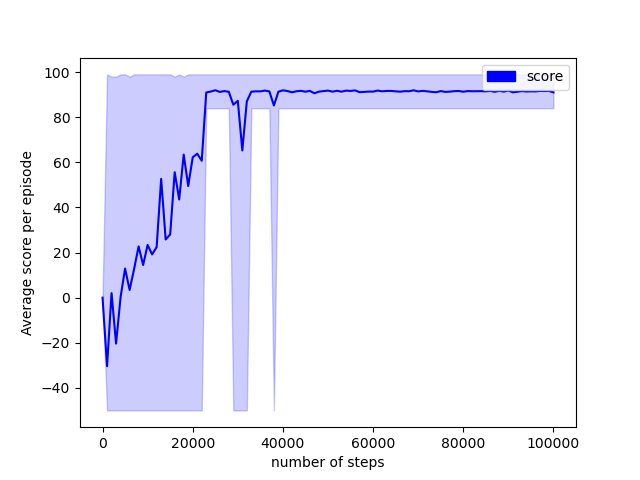
\includegraphics[width=7cm,height=6cm]{./code/performance.png}
	\caption{Q-Learning算法,开启阶梯学习率和经验回放,$\alpha=0.1,\gamma=0.8,replay\_size=100$。}
	\label{performance}
\end{figure}
平均累计奖励随样本训练量的增大而增大,并在平均奖励达到90左右时趋于稳定。并且模型的最小累计奖励可以维持在85左右。为了探究经验回放和阶梯学习率的作用,我还进行了如下对比实验。
\begin{figure}[h!]
	\centering
	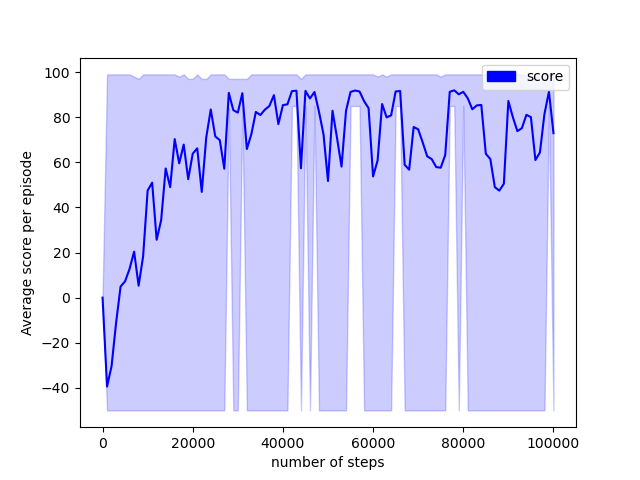
\includegraphics[width=7cm,height=6cm]{./code/performance_al=0.1_ga=0.8.png}
	\caption{Q-Learning算法,关闭阶梯学习率和经验回放,$\alpha=0.1,\gamma=0.8$。}
	\label{performance}
\end{figure}
\begin{figure}[h!]
	\centering
	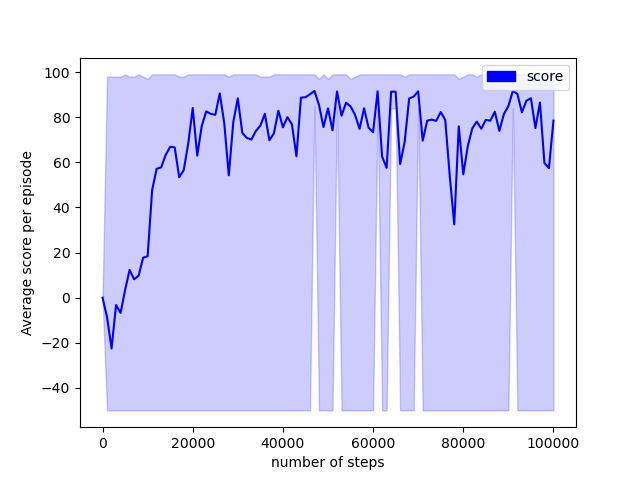
\includegraphics[width=7cm,height=6cm]{./code/performance_al=0.1_ga=0.8_rs=100.png}
	\caption{Q-Learning算法,关闭阶梯学习率,$\alpha=0.1,\gamma=0.8,replay\_size=100$。}
	\label{performance}
\end{figure}
\begin{figure}[h!]
	\centering
	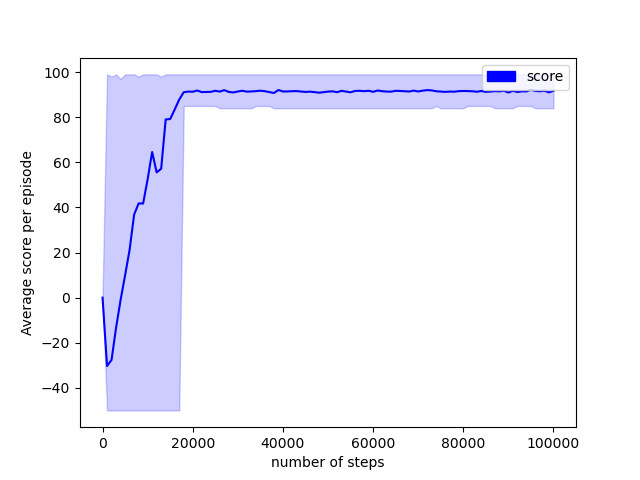
\includegraphics[width=7cm,height=6cm]{./code/performance_al=0.1_ga=0.8_laal=T.png}
	\caption{Q-Learning算法,关闭经验回放,$\alpha=0.1,\gamma=0.8$。}
	\label{performance}
\end{figure}
\section{小结}
在这次实验中,我发现由于Q-Learning算法不依赖专家知识,相较于Dagger算法实现更加方便,并且在gridworld环境中也能取得较好的效果。此外,通过对比实验我们可以发现,阶梯学习率能显著地提高模型的效果和训练速度,并且能够有效地稳定我们训练过程。相比之下,经验回放机制似乎能够提升模型的训练速度,但在当前参数设置下经验回放似乎没能够提升模型最终的效果或是稳定训练过程。因此在传统Q-Learning算法中,经验回放也许没能像它在QDN中那样有效。

\end{CJK}
\end{document}
